% Figure 1.5: Scaling Law Visualization
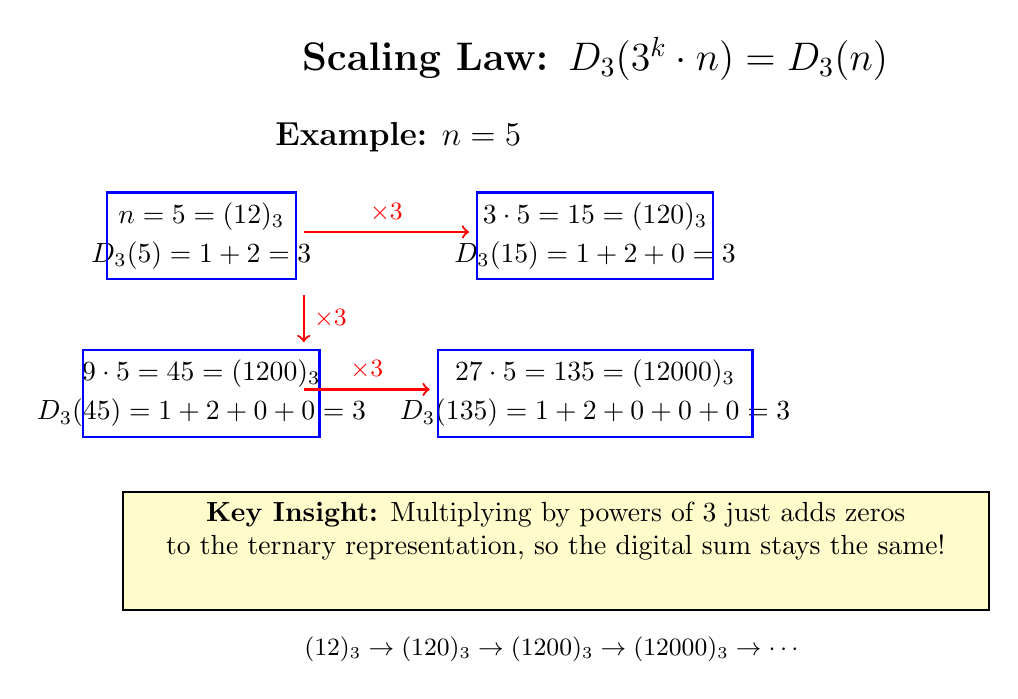
\begin{tikzpicture}[scale=1.0]

  % Title and main equation
  \node[font=\Large\bfseries] at (5,7.5) {Scaling Law: $D_3(3^k \cdot n) = D_3(n)$};

  % Example with n=5
  \node[font=\large, align=center] at (2.5,6.5) {\textbf{Example:} $n = 5$};

  % Show n=5
  \node[font=\normalsize] at (0,5.5) {$n = 5 = (12)_3$};
  \node[font=\normalsize] at (0,5.0) {$D_3(5) = 1 + 2 = 3$};
  \draw[thick, blue] (-1.2,4.7) rectangle (1.2,5.8);

  % Show 3·n = 15
  \node[font=\normalsize] at (5,5.5) {$3 \cdot 5 = 15 = (120)_3$};
  \node[font=\normalsize] at (5,5.0) {$D_3(15) = 1 + 2 + 0 = 3$};
  \draw[thick, blue] (3.5,4.7) rectangle (6.5,5.8);

  % Show 9·n = 45
  \node[font=\normalsize] at (0,3.5) {$9 \cdot 5 = 45 = (1200)_3$};
  \node[font=\normalsize] at (0,3.0) {$D_3(45) = 1 + 2 + 0 + 0 = 3$};
  \draw[thick, blue] (-1.5,2.7) rectangle (1.5,3.8);

  % Show 27·n = 135
  \node[font=\normalsize] at (5,3.5) {$27 \cdot 5 = 135 = (12000)_3$};
  \node[font=\normalsize] at (5,3.0) {$D_3(135) = 1 + 2 + 0 + 0 + 0 = 3$};
  \draw[thick, blue] (3.0,2.7) rectangle (7.0,3.8);

  % Arrows showing multiplication by 3
  \draw[->, thick, red] (1.3,5.3) -- (3.4,5.3) node[midway, above, font=\small] {$\times 3$};
  \draw[->, thick, red] (1.3,3.3) -- (2.9,3.3) node[midway, above, font=\small] {$\times 3$};
  \draw[->, thick, red] (1.3,4.5) -- (1.3,3.9) node[midway, right, font=\small] {$\times 3$};

  % Key insight box
  \draw[thick, fill=yellow!20] (-1,0.5) rectangle (10,2.0);
  \node[font=\normalsize, align=center] at (4.5,1.5) {
    \textbf{Key Insight:} Multiplying by powers of 3 just adds zeros\\
    to the ternary representation, so the digital sum stays the same!
  };

  % Visual representation
  \node[font=\small, align=center] at (4.5,0) {
    $(12)_3 \to (120)_3 \to (1200)_3 \to (12000)_3 \to \cdots$
  };

\end{tikzpicture}
